\begin{frame}\begin{center}
\LARGE\textbf{Instrumental Variables}
\end{center}\end{frame}
%-------------------------------------------------------------------------------
%-------------------------------------------------------------------------------
\begin{frame}\textbf{Key Identifiying Assumption}

\begin{align*}
(Y_1, Y_0)\indep Z\mid X\\
\end{align*}

Even in the best cases, this is sometimes not as obvious as you think. See \citeA{Heckman.1997c} for a study of implicit behavioral assumptions used in making program evaluations.
\end{frame}
%-------------------------------------------------------------------------------
%-------------------------------------------------------------------------------
\begin{frame}\textbf{Conventional Notation}

\begin{align*}
Y = \alpha + \beta D + \epsilon,
\end{align*}
where
\begin{align*}
\alpha &= \mu_0(X)  \\
\beta  & = (Y_1 - Y_0) =\mu_1(X) - \mu_0(X)  + (U_1 - U_0)\\
\epsilon & =U_0
\end{align*}
\end{frame}
%-------------------------------------------------------------------------------
%-------------------------------------------------------------------------------
\begin{frame}

Assume for now that there is no treatment effect heterogeneity, i.e. $Y_1 - Y_0$ is the same for everybody. If we have access to a variable $Z$ with the following properties ...

\begin{align*}
\cov(Z, D) & \neq 0 \\
\cov(Z, \epsilon) & = 0
\end{align*}

then the following holds

\begin{align*}
\plim \hat{\beta}_{IV} & = \frac{\cov(Z, Y)}{\cov(Z, D)} = \beta
\end{align*}
\end{frame}
%-------------------------------------------------------------------------------
%-------------------------------------------------------------------------------
\begin{frame}
What happens if $\beta$ varies in the population?\vspace{0.3cm}
\begin{itemize}\setlength\itemsep{1em}
\item Do individuals select their treatment status based on gains?\\\vspace{0.2cm}\hspace{0.3cm}$\Rightarrow$ essential heterogeneity
\end{itemize}
\end{frame}
%-------------------------------------------------------------------------------
%-------------------------------------------------------------------------------
\begin{frame}
Let $\beta = E[\beta] + \eta$, where $U_1 - U_0 = \eta$, then

\begin{align*}
Y = \alpha + \bar{\beta} D + [\epsilon + \eta D].
\end{align*}

and

\begin{align*}
\plim \hat{\beta}_{IV} & = \bar{\beta} + \frac{\cov(Z, \epsilon + \eta D)}{\cov(D, Z)}
\end{align*}

So we cannot even learn about the mean effect of treatment unless we rule out essential heterogeneity, i.e. individuals selecting their treatment status based on gains.
\end{frame}
%-------------------------------------------------------------------------------
%-------------------------------------------------------------------------------
\begin{frame}\textbf{Local Average Treatment Effect}
\begin{itemize}\setlength\itemsep{1em}
\item Average effect for those induced
to change treatment because of a change in the instrument.\\\vspace{0.2cm}
\(\Rightarrow\) instrument-dependent parameter\vspace{0.4cm}
\end{itemize}

\begin{align*}
&\frac{E(Y\mid Z = z) - E[Y \mid Z = z^\prime]}{P(z) - P(z^\prime)} = \\
 &\qquad E(Y_1 - Y_0\mid D(z) = 1, D(z^\prime) = 0)
\end{align*}

\end{frame}

%-------------------------------------------------------------------------------
%-------------------------------------------------------------------------------
\begin{frame}\begin{center}
\LARGE\textit{Local Instrumental Variables}
\end{center}\end{frame}
%-------------------------------------------------------------------------------
%-------------------------------------------------------------------------------
\begin{frame}\textbf{Local Instrumental Variable}

\begin{align*}
\left.\frac{\partial E(Y\mid P(Z) = p)}{\partial p}\right|_{p=u_D} & = E(Y_1 - Y_0 | U_D = u_D ) \\
        & =  B^{MTE} (u_D)
\end{align*}
$\Rightarrow$ we can only identify the $B^{MTE} (u_D)$ over the support of $p$ in our data
\end{frame}
%-------------------------------------------------------------------------------
%-------------------------------------------------------------------------------
\begin{frame}
\begin{figure}\caption{Observed Outcome and Essential Heterogeneity}
\scalebox{0.35}{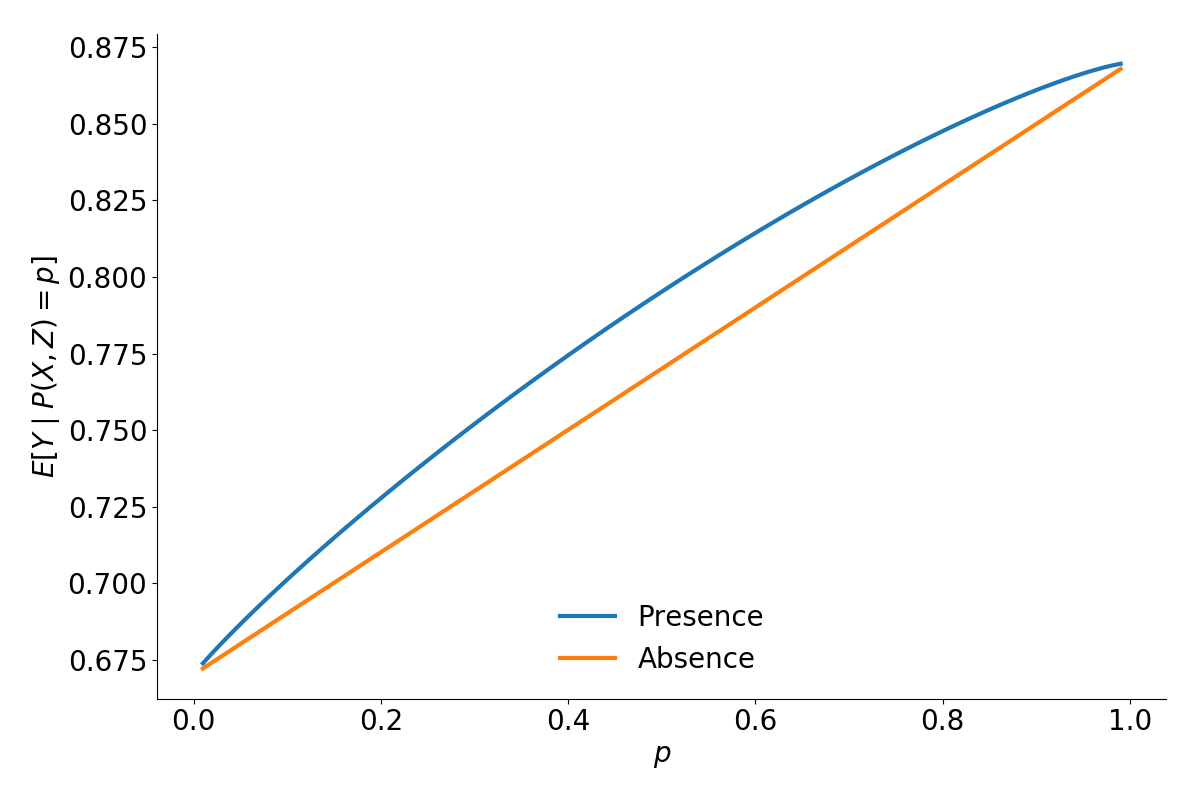
\includegraphics{fig-eh-conditional-expectation.png}}
\end{figure}
\end{frame}
%-------------------------------------------------------------------------------
%-------------------------------------------------------------------------------
\begin{frame}
\begin{figure}\caption{Identification I}
\scalebox{0.35}{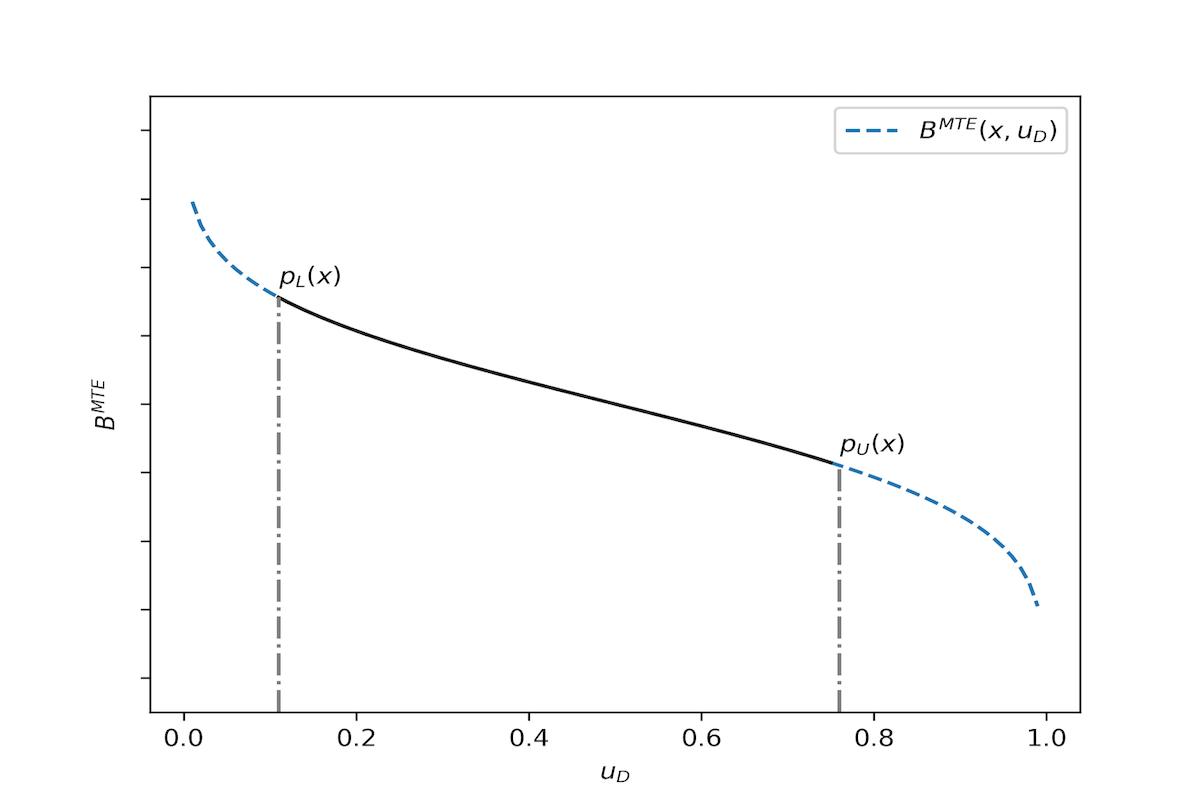
\includegraphics{fig-marginal-identification-single.png}}
\end{figure}
\end{frame}
%-------------------------------------------------------------------------------
%-------------------------------------------------------------------------------
\begin{frame}
Making $X = x$ explicit
\begin{align*}
 &E(Y_1 - Y_0 | X = x, U_D = u_D ) \\
 &\qquad= (\mu_1(x) - \mu_0(x)) + E(U_1 - U_0 | X = x, U_D = u_D )
\end{align*}
but if we are willing to assume $(U_1 - U_0)\indep X$ then
\begin{align*}
 &E(Y_1 - Y_0 | X = x, U_D = u_D ) \\
 &\qquad= (\mu_1(x) - \mu_0(x)) + E(U_1 - U_0 | U_D = u_D )
\end{align*}
\end{frame}
%-------------------------------------------------------------------------------
%-------------------------------------------------------------------------------
\begin{frame}
\begin{figure}\caption{Identification II}
\scalebox{0.35}{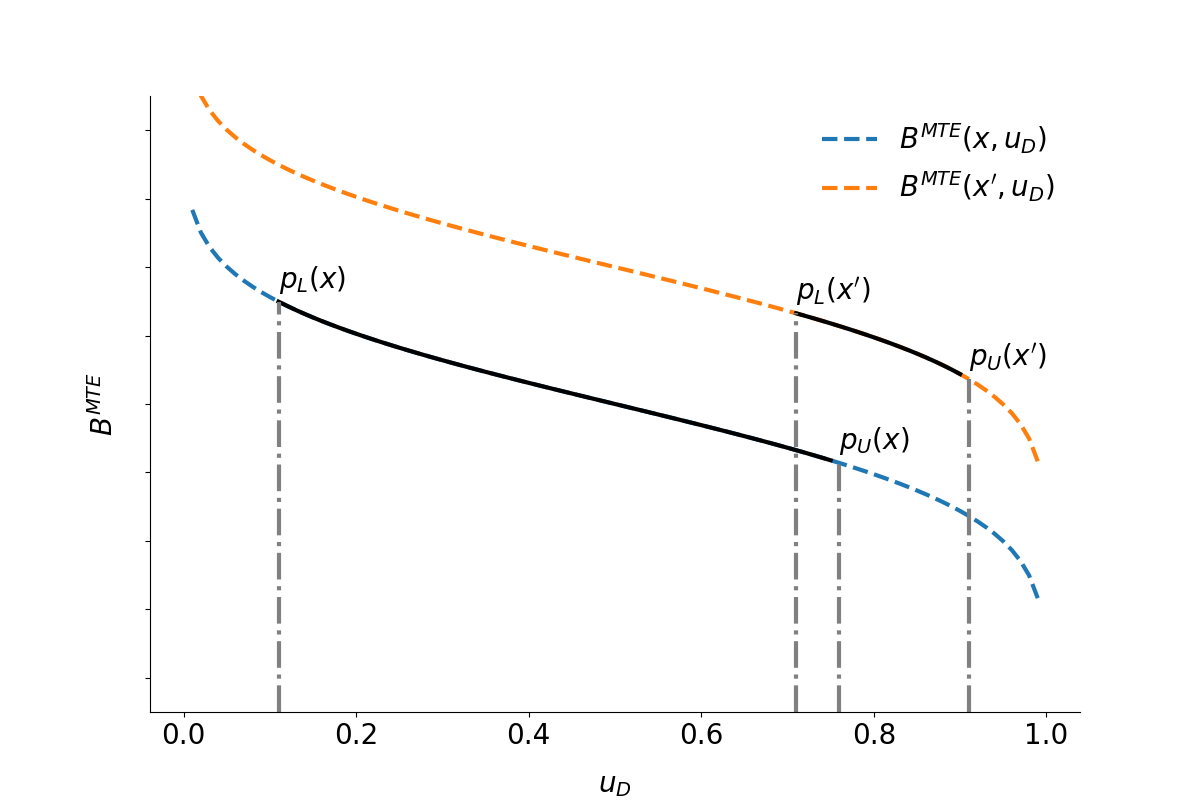
\includegraphics{fig-marginal-identification-double.png}}
\end{figure}
\end{frame}
%-------------------------------------------------------------------------------
%-------------------------------------------------------------------------------
\begin{frame}
\begin{figure}\caption{Identification III}
\scalebox{0.35}{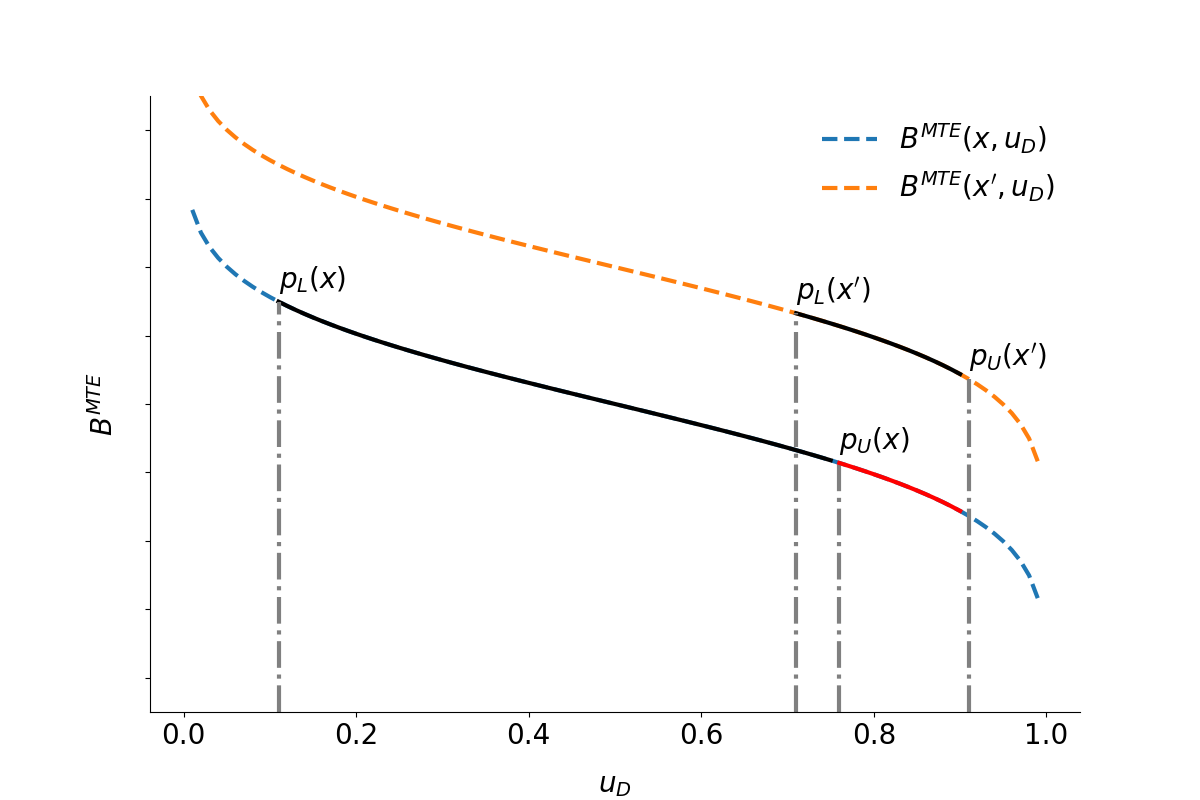
\includegraphics{fig-marginal-identification-combined.png}}
\end{figure}
\end{frame}
%-------------------------------------------------------------------------------
%-------------------------------------------------------------------------------
\begin{frame}
\textbf{Effects of Treatment as Weighted Averages}\vspace{0.3cm}

Parameter \(\Delta_j\), can be written as a weighted average of the
\(B^{MTE}(x, u_D)\).

\begin{align*}
\Delta_j(x) = \int_0^1 B^{MTE}(x, u_D) \omega^j(x, u_D) du_D,
\end{align*}

where the weights \(\omega^j(x, u_D)\) are specific to parameter \(j\)
and integrate to one.
\end{frame}
%-------------------------------------------------------------------------------
%-------------------------------------------------------------------------------
\begin{frame}
\begin{figure}\caption{Identification IV}
\scalebox{0.35}{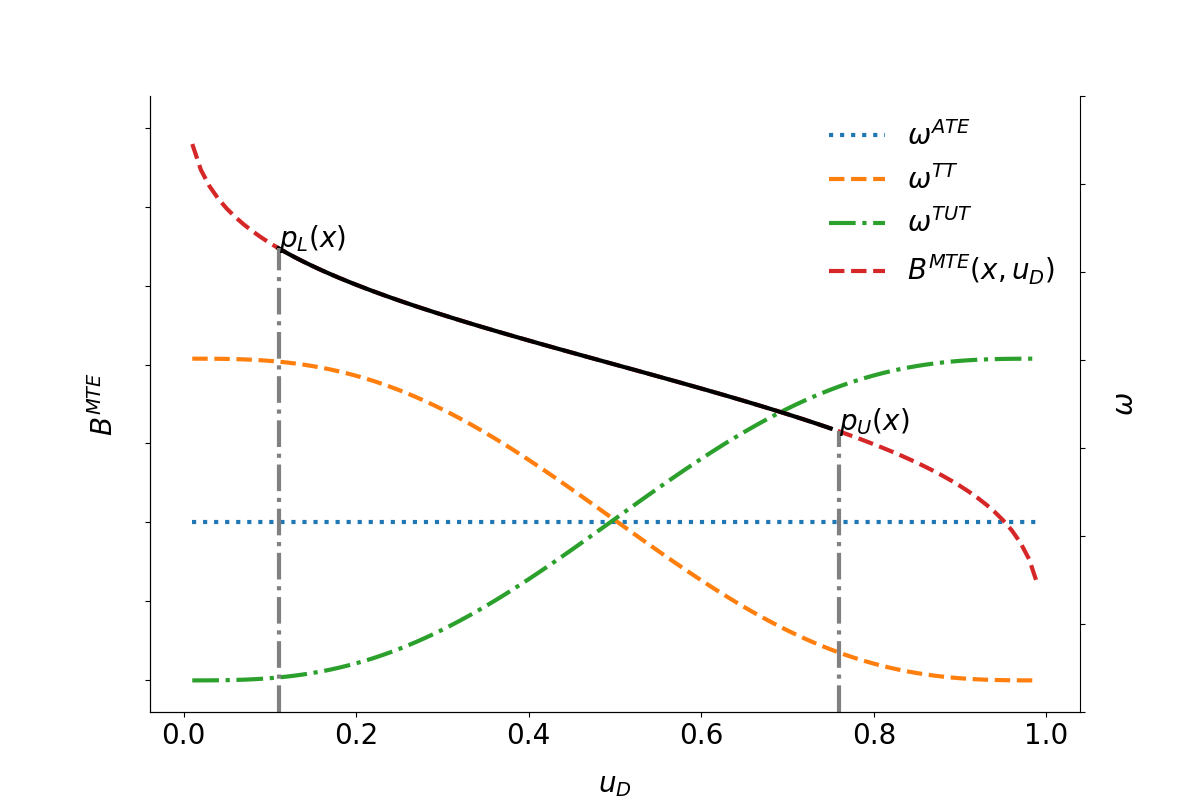
\includegraphics{fig-marginal-identification-weights.png}}
\end{figure}
\end{frame}
%-------------------------------------------------------------------------------
%-------------------------------------------------------------------------------
